%%% Verze pro jednostranný tisk:
\documentclass[11pt,a4paper]{report}
\usepackage[top=25mm,bottom=25mm,right=25mm,left=30mm,head=12.5mm,foot=12.5mm]{geometry}
\let\openright=\clearpage

%%% Pokud tiskneme oboustranně:
%\documentclass[11pt,a4paper,twoside,openright]{report}
%\usepackage[top=25mm,bottom=25mm,right=25mm,left=30mm,head=12.5mm,foot=12.5mm]{geometry}
%\let\openright=\cleardoublepage

%%% DEFINICE ZÁKLADNÍCH PROMĚNNÝCH
%\def\TypPrace{BP}                % bakalářská práce/bachelor thesis
\def\TypPrace{DP}               % diplomová práce/master thesis
%\def\Jazyk{cze}                  % čeština/czech
%\def\Jazyk{slo}                 % slovenština/slovak
\def\Jazyk{eng}                 % angličtina/english

%%% Definice různých užitečných maker (viz popis uvnitř souboru)
\input{makra}

\theoremstyle{remark}
\newtheorem*{remark}{Remark}


\theoremstyle{definition}
\newtheorem{definition}{Definition}[chapter]

\newtheorem{theorem}{Theorem}[chapter]
\newtheorem{lemma}{Lemma}[theorem]

\DeclareMathOperator{\src}{s}
\DeclareMathOperator{\tar}{t}
\DeclareMathOperator{\indeg}{d_{in}}
\DeclareMathOperator{\outdeg}{d_{in}}
\DeclareMathOperator{\inedges}{\delta_{in}}
\DeclareMathOperator{\outedges}{\delta_{out}}
\DeclareMathOperator{\inver}{N_{in}}
\DeclareMathOperator{\outver}{N_{out}}

\usepackage{color}
\usepackage{listings}
\usepackage{caption}

\newcounter{nalg}[chapter] % defines algorithm counter for chapter-level
\renewcommand{\thenalg}{\thechapter .\arabic{nalg}} %defines appearance of the algorithm counter

\DeclareCaptionLabelFormat{algocaption}{Algorithm \thenalg} % defines a new caption label as Algorithm x.y
\lstnewenvironment{algorithm}[1][] %defines the algorithm listing environment
{   
    \refstepcounter{nalg} %increments algorithm number
    \captionsetup{labelformat=algocaption,labelsep=colon} %defines the caption setup for: it ises label format as the declared caption label above and makes label and caption text to be separated by a ':'
    \lstset{
        mathescape=true,
        frame=tB,
        % numbers=left, 
        % numberstyle=\tiny,
        basicstyle=\small, 
        keywordstyle=\color{black}\bfseries\em,
        keywords={,input, output, return, datatype, function, is, in, if, else, foreach, while, for, begin, end, } %add the keywords you want, or load a language as Rubens explains in his comment above.
        xleftmargin=.04\textwidth,
        #1 % this is to add specific settings to an usage of this environment (for instnce, the caption and referable label)
    }
}
{}

\colorlet{punct}{red!60!black}
% \definecolor{background}{HTML}{EEEEEE}
\definecolor{delim}{RGB}{20,105,176}
% \colorlet{numb}{magenta!60!black}

\colorlet{punct}{red!60!black}

\DeclareCaptionLabelFormat{datacaption}{Data \thenalg} % defines a new caption label as Algorithm x.y
\lstnewenvironment{data}[1][] %defines the algorithm listing environment
{   
    \refstepcounter{nalg} %increments algorithm number
    \captionsetup{labelformat=datacaption,labelsep=colon} %defines the caption setup for: it ises label format as the declared caption label above and makes label and caption text to be separated by a ':'
    \lstset{ %this is the stype
        frame=tB,
        basicstyle=\footnotesize\ttfamily,
        literate=
           *{:}{{{\color{punct}{:}}}}{1}
            {,}{{{\color{punct}{,}}}}{1}
            {\{}{{{\color{delim}{\{}}}}{1}
            {\}}{{{\color{delim}{\}}}}}{1}
            {[}{{{\color{delim}{[}}}}{1}
            {]}{{{\color{delim}{]}}}}{1},
        #1
    }
}
{}

\bibliography{00references.bib}

%%% Název práce v jazyce práce (přesně podle zadání)
%%% Title of the thesis in the language used in the text (exact according to assignment)
\def\NazevPrace{Heuristics for real-time train dispatching}

%%% Jméno autora
%%% Author's name - First name Surname
\def\AutorPrace{Ing. Bc. Jan Švrčina}

%%% Rok odevzdání a měsíc (slovně)
%%% Year of submission and month (verbally) - month YYYY
\def\DatumOdevzdani{May 2026}

%%% Vedoucí práce: Jméno a příjmení s~tituly
%%% Supervisor: First name and surname with titles
\def\Vedouci{Ing. Miroslav Rada, Ph.D.}

%%% Konzultant práce: Jméno a příjmení s~tituly
%%% Consultant: First name and surname with titles
\def\Konzultant{}

%%% Studijní program
%%% Study program
\def\StudijniProgram{Econometrics and Operations Research}

%%% Studijní program - specializace
%%% Study program - specialization
\def\Specializace{}

%%% Nepovinné poděkování (vedoucímu práce, konzultantovi, tomu, kdo zapůjčil software, literaturu apod.)
%%% Optional thanks (the supervisor, the consultant, the borrower of software, literature, etc.)
\def\Podekovani{%
I thank my supervisor for his patience and the assistance he provided, my alma mater for~the~knowledge and connections it has given me, and my mother for the lifelong support of my education.
}


%%% Abstrakt (doporučený rozsah cca 150-250 slov; nejedná se o zadání práce)
% LTex: language=cs
\def\Abstrakt{%
\begin{otherlanguage}{czech}
Tato práce se zabývá problémem dispečerského řízení vlaků (TDP) a návrhem heuristiky schopné rozhodování v reálném čase pro komplexní železniční sítě. Naše metoda využívá přístup shora dolů pro rozhodování o trasování, motivovaný strukturní analýzou instancí, včetně bezpečnostních hledisek, a formulací pomocí cest a cyklů pro řešení konfliktů, což odstraňuje nutnost používat omezení s velkým M.

Procedury pro trasování i řešení konfliktů vycházejí z efektivního agregačního postupu a inovativní struktury grafu propojení (link graph). Agregační postup zmenšuje velikost problému a lze jej využít pro jakoukoli rozvrhovací úlohu s alokací zdrojů. Graf propojení uchovává informace o závislostech zdrojů pro aktuální výběr tras a umožňuje nám vytvářet strukturní implikační pravidla, která lze použít k identifikaci kritických částí při rozhodování o trasování a ke snížení počtu požadovaných proměnných a omezení při řešení konfliktů.

Heuristika byla použita k vyřešení většiny instancí v knihovně benchmarků DISPLIB a přinesla výrazné zlepšení rychlosti ve srovnání s vítěznými řešeními, i když za cenu občasných suboptimálních řešení. Výsledky jasně ukazují výhody a nevýhody formulace cest a cyklů a ilustrují, jak se struktura grafu propojení využívá v praxi.
\end{otherlanguage}
}

% LTex: language=en-US
\def\AbstraktEN{%
This thesis addresses the train dispatching problem (TDP) by creating a heuristic capable of real-time decision-making for complex railway networks. Our method uses a top-down approach for routing decisions, motivated by structural analysis of the instances, including safety concerns, and a path-and-cycle formulation for conflict resolution, which removes the~need to use big-M constraints.

Both routing and conflict resolution are based on an efficient aggregation procedure and~an~innovative link graph structure. The aggregation procedure reduces the problem size and can be utilized for any scheduling problem with resource allocation. The link graph maintains the information about resource dependencies for the current route selection and allows us to~create structural implication rules which can be used to identify critical parts when making routing decisions, and to~reduce the number of required variables and constraints for conflict resolution.

The heuristic was used to solve the majority of the instances in the DISPLIB benchmark library and provided a significant improvement in speed compared to the winning solutions, albeit at the cost of sometimes suboptimal solutions. The results clearly demonstrate the~advantages and drawbacks of the path-and-cycle formulation, and illustrate how the link graph structure is used in practice.
}



%%% 3 až 5 klíčových slov (doporučeno)
\def\KlicovaSlova{klíčové slovo, další pojem, jiný důležitý termín, a ještě jeden}
\def\KlicovaSlovaEN{keyword, important term, another topic, and another one}



%%% Titulní strana a různé povinné informativní strany
%%% Title page and various mandatory information pages
\begin{document}
% \include{01title}

\pagestyle{fancyx}
%%% Jednotlivé kapitoly práce jsou pro přehlednost uloženy v samostatných souborech
%%% The individual chapters of the thesis are stored in separate files for clarity
{%
\pagestyle{plain}
% %%% Strana s automaticky generovaným obsahem práce
%%% A page with automatically generated content of the thesis
\setcounter{tocdepth}{2}
\tableofcontents

%%% Seznam obrázků v práci
%%% List of figures in the thesis
\openright
\listoffigures
Poznámka: Seznam obrázků je vhodné použít, pokud počet obrázků v textu práce je větší než 20.

%%% Seznam tabulek v práci (volitelně)
%%% List of tables in the thesis (optionally)
\clearpage
\listoftables
Poznámka: Seznam tabulek je vhodný použít, pokud počet tabulek v textu práce je větší než 20.

%%% Seznam zdrojových kódů v práci (volitelně)
%%% List of source listings in the thesis (optionally)
\clearpage
\lstlistoflistings
Poznámka: Seznam výpisů programového kódu je vhodné použít, pokud počet vložených objektů tohoto typu je větší než 20. 

%%% Seznam zkratek v práci (volitelně)
%%% List of abbreviations in the thesis (optionally)

% \include{03shortcut}
% \include{doporuceni}
% \include{uvod}
}

\chapter{Introduction}
\label{chap:intro}

\section{Motivation}

Railway transportation remains relevant even after its long history due to its efficiency, safety, and~sustainability. However, the~most limiting factor has always been the~use of~the required infrastructure. As such, the~critical problem of~utilizing the~railway effectively has always been scheduling. The complexity of~this problem is continuously increasing with the~size and~intricacy of~the railway system as well as the~demand to use it. 

Traditionally, scheduling was done manually by humans; only with the~advancements of~optimizing algorithms and~computational power have humans been aided by computers. This still produces a static schedule that might be unusable if a disruption occurs. This is where train dispatching comes into play where the~decisions are made in~real-time, managing delays and~conflicts as they happen. Real-time dispatching is often still only done by humans and~provides a challenge for~optimization algorithms as they need to find an acceptable solution in~a matter of~minutes or~even seconds.

\section{Goals}
The main goal of~this thesis is to develop a heuristic that is capable of~train dispatching in~real-time with interpretable results; a human should be able to understand the~structure of~the result to verify its validity.

The heuristic will be evaluated on~the \emph{DISPLIB}\@: Train dispatching benchmark library \cite{kloster2025displiblibrarytraindispatching} consisting of~train dispatching problem (TDP) instances from real-world data. This library of~instances was introduced for~an optimization competition.

A significant part of~this thesis is focused on~the aggregation of~the problem as presented in~the \emph{DISPLIB}. This is the~main innovation which allows us to use a top-down approach, reducing the~problem into selecting the~routes top-down and~then scheduling it with a more concise model, as opposed to the~bottom-up approach, building up the~solutions by sequentially routing and~resolving conflicts, which is used by the~winning solutions in~the \emph{DISPLIB} competition.

\section{Thesis structure}
\begin{minipage}{\textwidth}
This thesis is structured in~the following chapters with their contents:

\begin{enumerate}
	\item \hyperref[chap:intro]{\emph{Introduction:}} Outlines the~motivation, goals and~structure of~this thesis.
	%\hyperref[chap:lit_rev]
	\item \hyperref[chap:lit_rev]{\emph{Literature review:}} Review of~the pertinent literature separated into three parts, literature connected to the~\emph{DISPLIB}, the~most relevant resources inspiring the~heuristic or~providing key theoretical ideas, and~an overview of~selected state-of-the-art in~scheduling optimization.
	\item \hyperref[chap:theor]{\emph{Theoretical background:}} Basic theory necessary for~the description of~the problem. The~main focus is on~graph topology and~the use of~alternative and~disjunctive graphs for~scheduling models.
	\item \hyperref[chap:method]{\emph{Methodology:}} Detailed description of~the problem, aggregation, routing and~conflict resolution.
	\item \hyperref[chap:results]{\emph{Results:}} Presentation of~performance of~the algorithms described in~methodology on~the~\emph{DISPLIB} instances.
	\item \hyperref[chap:discuss]{\emph{Discussion:}} Discussion of the ideas and procedures presented in the methodology chapter and discussion of~results.
	\item \hyperref[chap:concl]{\emph{Conclusion:}} Highlight of~main ideas presented in~this thesis and overall evaluation, future work considerations.
\end{enumerate}
\end{minipage}



\chapter{Literature review}


This chapter provides a review of the relevent literature separated into 3 parts. First is literature revelent to the \emph{DISPLIB}. Second are the most revelevant resources inspiring the heuristic or providing key theoretical ideas. Third is an overview of selected state of the art in scheduling optimization.

\section{DISPLIB}

As the main goal of this thesis is to make a heuristic that solves instances from the \emph{DISPLIB} library, we provide a review of the introductory paper as well as a description of the competiton winning solutions.

\subsection{Problem and library}
The train dispatching problem (TDP) which this thesis is working with is presented in \emph{DISPLIB: A library of train dispatching problems } \cite{kloster2025displiblibrarytraindispatching} alongside the collection of instances which can be used to benchmark this problem. This provides an imporant step for the subfield of train dispatching optimization - a unified problem format and real-life data to be used for benchmarking. The instances and competition results can be accesed from~\url{https://displib.github.io/}.

\blockcquote{kloster2025displiblibrarytraindispatching}{
	... each study (on train scheduling) is typically tightly connected with a specific industrial use case. Code and data are seldom shared publicly. This fact hinders reproducibility, and has led to a proliferation of papers describing algorithms for more or less compatible problem definitions, without any real opportunity for readers to assess their relative performance. Inspired by the successful communities around MILP, SAT, TSP, VRP, etc., we introduce a common problem definition and file format, \emph{DISPLIB}, which captures all the main	features of train re-routing and re-scheduling.
}

The instances are published with best known solutions (assumed with unlimited time), unfortunatelly for the 10 minute computation time limit only the competition team rankings are presented, without overview of the actual solutions.

\subsection{Competition and solutions}
Part of the presentation of \emph{DISPLIB} was also the anouncement of the competition for optimization using this library. The competition concluded at the Optimization and Decision Science Conference (ODS) 2025 where they presented the winners. Unfortunatelly the materials for the solutions are not available and only one team wrote a paper about their solution. Still, we find essential to provide the reader with the description for other solutions, so the limited information from the book of abstracts for the ODS 2025 \cite{ods2025bookofabstracts} is summarized.

The first place went to Carolin Scholl and Luka Stärk (DB Systel GmbH). Their solution is based on branch and bound inspired by Monte Carlo Tree Search \cite{DARIANO2007643}, prioritizing not only lower bound improvement but also search for feasible solutions. In each step of the tree they resolve the chronologacally first conflict either by setting precedence to either of the trains on the conflicting resources or by rerouting either train if possible. This is a bottom-up approach, only adding the necessary constrains for current conflicts.

The second place went to Openbus team (ETH Zürich) which published a description of their solution in \emph{Handling Conflicts in Microscopic Railway Timetabling at Scale: A Hybrid Approach}\footnote{This paper is not officially published, only a pre-print was available.} \cite{Dubach2025handling}. Their solution utilizes 2 distinct solvers which run in parallel. First one is a Logic-Based Benders Decomposition (LBBD) procedure \cite{Leutwiler2022logic} where a master mixed-integer programing (MIP) problem performs a selection of current available paths, slave satisfiability modulo theory (SMT) solver creates a feasible time table if possible (without conflicts) and a subproblem detects conflicts and adds them SMT solver, which in turn adds cuts to the master problem to maintain feasiblity. Figure \ref{fig:openbus_lbbd} show the diagram of the solver as presented in their poster. Second solver uses a simpler MIP representation which iteratively relaxes the bounds for conflicing resources and tightens the bounds for non-conflicing resources converging to a feasible solution. Both of these solvers use a bottom-up approach, after a bound tightening procedure is applied globally. The authors argue that both of these solvers exploit different instance structures and share their bounds to improve convergence.

\begin{figure}[htbp!]
\caption{Openbus DISPLIB competition poster}
\label{fig:openbus_lbbd}
\begin{center}
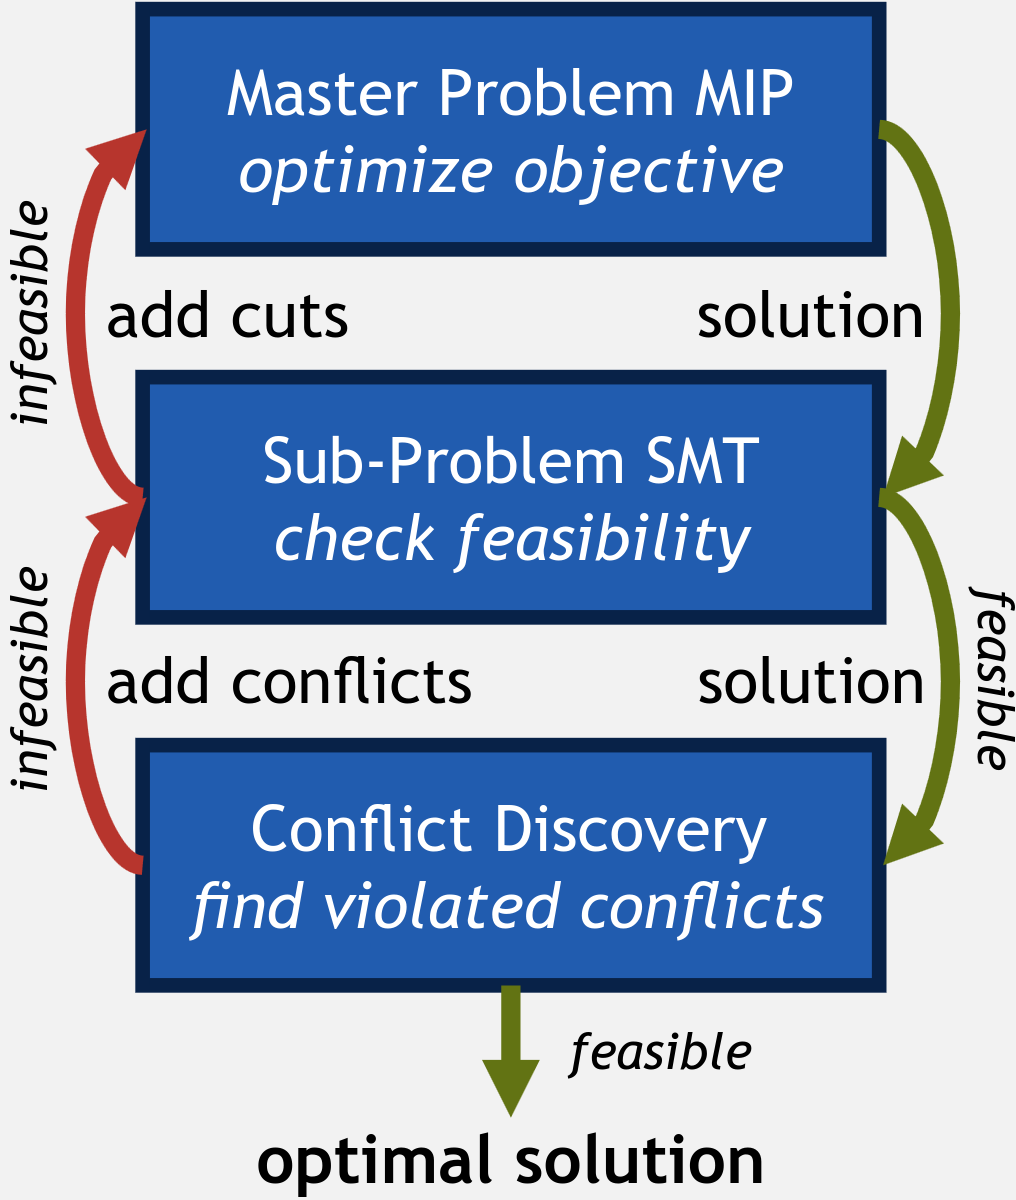
\includegraphics[width=.525\textwidth]{img/openbus_lbbd.png}
\end{center}

\footnotesize \textit{Source:} ETH Zürich Research Collection \cite{Dubach2025poster}
\end{figure}

The third place went to Venislav Steliyanov Varbanov (independent). This solution also uses an MIP model with a decomposition to reduce the number of time variables - this idea is also used by the heuristic in this thesis, inspired by the provided description. After this aggregation of time variables, the conflicts are again resolved sequentially, similarly to the other 2 solutions.

We can see that while the winning solutions may differ in their model representation and optimization approach, and 2 of them use a certain level of aggregation, they have one thing in common - they resolve the conflicts sequentially and thus they only need to consider the conflicts that arise in the current partial solution and therefore the number of constrains and variables necessary to prevent the conflicts stays limited.

\section{Theory and heuristics}

While the \emph{DISPLIB} winning solutions provided us with the ideas of aggregation of variables and combining conflict resolutions, it provided very little on the actual implementation. This section descibes the relevant sources to explain the necessary theory to model the problem effectively.

Referenced by the winning solution is \emph{A Branch and Bound Algorithm for Scheduling Trains in a Railway Network} \cite{DARIANO2007643}. It uses an alternative graph formulation for the train scheduling problem. With this representation we can model resouce conflicts with alternative precedence arcs. It also describes the idea of inferred selection, meaning that by choosing one precence alternative for a resource implies selection on another resources (the alternative is forbidden as it would produce an infeasible solution).

\emph{Job-shop Scheduling with Blocking and No-wait Constraints} \cite{MASCIS2002498} introduces the alternative graph concept as a generalization of the disjunctive graph \cite{roy1964problemes}. The alternative graph is used to formulate a model for the blocking job-shop problem (BJSP) that is closely related to TDP.

\emph{Improving Real-Time Train Dispatching: Models, Algorithms and Applications.} \cite[p. 84-85]{dariano2008improving} provides static implication rules for the alternative graph representation that can be used for inferred selection based on the structure of TDP.

\emph{Railway scheduling problems and their decomposition} \cite{Strotmann2007} is thesis that show decomposition techniques that inspired the decomposition used in this thesis to split the global problem into small subgraphs using border operations and a global synchronizer to merge the solution from these subgraphs and deal with potention conflicts.

\section{State of the art}
Because the description of the solutions that are directly connected to this thesis is limited, we provide the reader with an overview of the recent state of the art solutions for closely related problems in train dispatching and scheduling.

\emph{Optimizing train dispatching for the Union Pacific Railroad}~\cite{boccia2025optimizing} presents an automated dispatching system that is in use on a real rail network. It uses a decomposition of the problem and global synchronizer to resolve conflict. It is a prime example how optimization can improve real-life solutions.

\emph{A Branch-and-Cut Algorithm for Scheduling Train Platoons in Urban Rail Networks}~\cite{chai2024branch} describes a mixed-integer linear problem (MILP) for scheduling of train platoons, problem where different vehicles are flexibly and dynamically coupled and decoupled.

Authors in \emph{Decentralised Multi-Agent Coordination for Real-Time Railway Traffic Management} \cite{damato2025decentralised} propose the use of another emerging idea - instead of central or area based decomposition schedulers, trains cooperate as separate agents to prevent conflicts and achieve efficient scheduling. This decentralized nature of cooperation has already been used on drone related problems with success \cite{HertJINTHW_paper}.



\chapter{Theoretical background}

This chapter will cover the necessary theory used to formulate and solver our problem. Main focus will be on graph topology and alternative graphs and their relation to the train dispatching problem. 

\section{Basic definitions}
While some of these definitions may feel redundant, we will use them as an opportunity to establish the notation. Most of the definitions are paraphrased from \emph{Handbook of Graph Theory} \cite{gross2013handbook} with notation adjusted to ours.


\begin{definition}
Graph is an ordered pair $G = (V,\ E)$, where $V = \{v_i\}_{i=1}^{n_v}$ is a set vertices \footnote{\label{note:nodes}Vertices are often called nodes.} and $E = \{e_i\}_{i=0}^{n_e}$ is a set of edges, where edge $e = \{u,\ v\},\ u,\ v \in V$ is an \emph{unordered} pair of vertices.
\end{definition}

\begin{definition}
\label{def:digraph}
Directed graph (digraph) is an ordered pair $G = (V,\ E)$, where $V = \{v_i\}_{i=1}^{n_v}$ is a set vertices and $E = \{e_i\}_{i=0}^{n_e}$ is a set of edges \footnote{\label{note:arcs}Commonly the edges in directed graphs are called arcs.}, where edge $e = (u,\ v),\ u,\ v \in V$ is an \emph{ordered} pair of vertices.
\end{definition}


\begin{definition}
Multigraph is an ordered tuple $G = (V,\ E,\ r)$, where $V = \{v_i\}_{i=1}^{n_v}$ is a set vertices, $E = \{e_i\}_{i=0}^{n_e}$ is a set of edges and $r:\ E \rightarrow \{\{u,\ v\}\ |\ u,\ v \in V\}$ is a mapping from edges to pair of endpoint vertices.
\end{definition}

\begin{definition}
Directed multigraph is an ordered tuple $G = (V,\ E,\ s,\ t)$, where $V = \{v_i\}_{i=1}^{n_v}$ is a set vertices, $E = \{e_i\}_{i=0}^{n_e}$ is a set of edges and $s:\ E \rightarrow V$ is a source (start) mapping from edges to vertices and $t:\ E \rightarrow V$ is a target (end) mapping from edges to vertices.
\end{definition}


Example of each type of graph is in figure \ref{fig:graph_example}.

\begin{remark}
As you can see in figure \ref{fig:graph_example}, digraph allows for parallel edges (2, 3) and (3, 2). This will be a useful property for the alternative graph definition.
\end{remark}

\begin{figure}[htbp!]
\caption{Example of graph (A), digraph (B), multigraph (C) and directed multigraph (D)}
\label{fig:graph_example}
\begin{center}
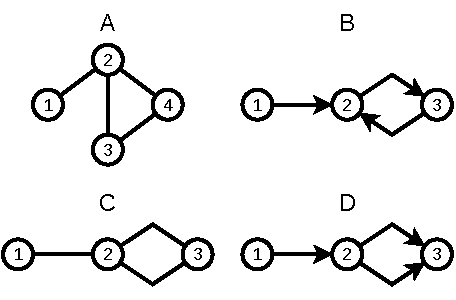
\includegraphics[width=.8\textwidth]{img/graph_example.pdf}
\end{center}
\end{figure}

Since we will mostly be working with directed graph, to following definitions are tailored for directed graphs. The following definitions of operators also abuse the notation by ommiting the specification of graph $G$, which will be included in the context of multiple graphs if necessary.

\begin{definition}
Source (start) $\src(e) = u,\ e = (u,\ v)$ is the starting vertex of edge $e$.
\end{definition}

\begin{definition}
Target (end) $\tar(e) = v,\ e = (u,\ v)$ is the ending vertex of edge $e$.
\end{definition}

\begin{definition}
Incomming edges $\inedges(v) = \{e\ |\ t(e) = v,\ e \in E\}$ of vertex $v$ is a set of edges $e$ that end in $v$.
\end{definition}

\begin{definition}
Outgoing edges $\outedges(v) = \{e\ |\ s(e) = v,\ e \in E\}$ of vertex $v$ is a set of edges $e$ that start in $v$.
\end{definition}

\begin{definition}
Predecessors (In-neighborhood) $\inver(v) = \{u\ |\ u = \src(e),\ e \in \inedges(v)\}$ of vertex $v$ is a set of vertices $u$ that are connect to $v$ via its incomming edges.
\end{definition}

\begin{definition}
Successors (Out-neighborhood) $\outver(v) = \{w\ |\ w = \tar(e),\ e \in \outedges(v)\}$ of vertex $v$ is a set of vertices $w$ that are connect to $v$ via its outgoing edges.
\end{definition}

\begin{definition}
In-degree $\indeg(v) = |\inedges(v)|$ is the number of incomming edges of $v$.
\end{definition}

\begin{definition}
Out-degree $\outdeg(v) = |\outedges(v)|$ is the number of incomming edges of $v$.
\end{definition}

\begin{definition}
Path is $P = \mathrm{P}(u,\ v)$ from $u$ to $v$ is a sequence of edges $(e_i)_{i=1}^N$, such that $\tar(e_{i-1}) = \src(e_i),\ 2 \leq i \leq n$, $u = src(e_0)$ and $v = \tar(e_n)$.
\end{definition}

\begin{definition}
Cycle is a path that starts and ends in the same vertex.
\end{definition}

\section{Graph topology}
\begin{definition}
Directed acyclic graph (DAG) is directed graph that contains no cycle.
\end{definition}

\begin{definition}
Topological order is a sequence of vertices in directed graph $(v_i)_{i=1}^{|V|}$ such that $e = (u, v) \implies u \prec v$ ($u$ apears before $v$ in the sequence).
\end{definition}

\begin{theorem}
Topological order can only be created for acyclic graphs.
\end{theorem}

\begin{proof}
By contradiction, for path starting at $u$ and ending at $v$, $u \prec v$ in the topological order, because for each $e = (x, y)$ in path, $x \prec y$ and ordering $\prec$ is transitive. For cycle $u$ and $v$ are in the same spot in the order, this is a contradiction.
\end{proof}

To detect a cycle and get a topological sort we use algorithm \ref{alg:toposort}, it is acombination for depths first search (DFS) for cycle detection and DFS for topological sorting \cite{CLRS2022}. It runs in $\mathrm{O}(|V| + |E|)$ time complexity with $\mathrm{O}(|V|)$ required space. It allows us to do both cycle detection and topological sort in one pass of DFS.

\begin{algorithm}[float, caption={Topological sort with cycle detection}, label={alg:toposort}]
input: graph G
output: () if G contains cycle else topological order of G

function: DFS(v, label, stack)
  if label(v) is InRecursion
    return true
  else if label(v) is Done
    return false
  end

  label(v) $\gets$ InRecursion

  foreach s $\in \outver$(v)
    if DFS(s, label, stack)
      return true
    end
  end

  stack.push(v)
  label(v) $\gets$ Done

  return false
end

begin
  foreach v $\in$ V(G)
    label(v) $\gets$ NotDone
  end

  stack $\gets$ EmptyStack

  foreach v $\in$ V(G)
    if DFS(v, label, stack)
      return ()
    end
  end

  order $\gets$ reverse(stack)
  return order
end
\end{algorithm}


\section{Alternative graphs}

Alternative graphs were introduced in \cite{MASCIS2002498}. The provide a very useful framework for modeling resource allocation problems with blocking. They are a generalization of disjunctive graphs \cite{roy1964problemes}.

\begin{definition}
Alternative graph is an ordered tuple $G = (V,\ E,\ A)$, where $V = \{v_i\}_{i=1}^{n_v}$ is a set vertices, $E = \{e_i\}_{i=0}^{n_e}$ is a set edges $e = (u,\ v),\ u,\ v \in V$, and $A = \{a_i\}_{i=0}^{n_a}$ is a set of disjunctive (alternative) edge pairs $a = ((u,\ v),\ (x,\ y)),\ u,\ v,\ x,\ y \in V$.
\end{definition}

\begin{remark}
We denote the alternative $\bar{e}$ to the edge $e$ from the disjunctive pair $a = (e,\ \bar{e})$.
\end{remark}

To illustrate the concept of alternative graphs, figure \ref{fig:alt_graph_example} shows an altertative graph with 3 disjunctive pairs.

\begin{figure}[htbp!]
\caption{Example of alternative graph}
\label{fig:alt_graph_example}
\begin{center}
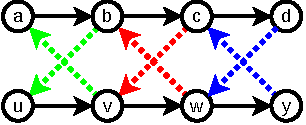
\includegraphics[width=0.6\textwidth]{img/alt_graph_example.pdf}
\end{center}
\end{figure}

\begin{definition}
A selection $S$ is a set of edges obtained by from $A$ by choosing at most one edge from each pair. The edges in this selection are selected, their alternatives (the other edge from the pair) is forbidden. 
\end{definition}

\begin{definition}
Selection $S$ is complete if exactly one edges is chosen from each pair, otherwise its a partial selection. 
\end{definition}

\begin{definition}
Selection $S$ is consistent if graph $(V,\, E \cup S)$ does not contain a cycle. If the graph does contain a cycle, the selection is inconsistent.
\end{definition}

To illustrate the selection terms, figure \ref{fig:alt_graph_selection} shows different types of selections from on alternative graph from figure \ref{fig:alt_graph_example}.

\begin{figure}[htbp!]
\caption{Examples for partial inconsistent (A), partial consistent (B), complete inconsistent (C), and complete consistent (D) selections}
\label{fig:alt_graph_selection}
\begin{center}
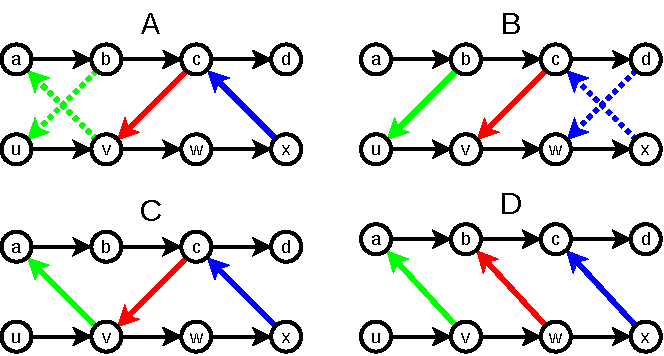
\includegraphics[width=1.0\textwidth]{img/alt_graph_selection.pdf}
\end{center}
\end{figure}

\begin{definition}
Alternative edge $e$ is inferred from selection $S$, $S \vdash e$ if $S \cup \{\bar{e}\}$ is an inconsistent selection, meaning that the choice of $e$ from altertative pair $(e,\ \bar{e})$ can be inferred from $S$ because choosing $\bar{e}$ would be inconsistent. Similarly we can say that one alternative edge $x$ implies another $y$, $x \implies y$ if $\{x\} \vdash y$.
\end{definition}


An example from on graphs in figure \ref{fig:alt_graph_example}, we can see that $(b,\ u) \implies (c,\ v)$ and $(v,\ a) \implies (w,\ b)$ etc.

\begin{remark}
It is possible to have a partial consistent selection $P$ for which there exist no complete consistent complete selection $C$, $P \subset C$. One such case is in figure \ref{fig:alt_graph_infeasible}, where $(b,\ u) \implies (c,\ v)$ and $(x,\ c) \implies (w,\ b)$. Beacuse $(c,\ v)$ and $(w,\ b)$ are in the same disjunctive pair, we cannot make a consistent selection for this pair.
\end{remark}


\begin{figure}[htbp!]
\caption{Examples of partial consistent selection without possible complete consistent selection}
\label{fig:alt_graph_infeasible}
\begin{center}
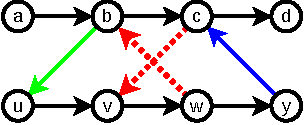
\includegraphics[width=.6\textwidth]{img/alt_graph_infeasible.pdf}
\end{center}
\end{figure}

\subsection{Weighted graphs}

To extend the descriptive ability of graphs to model problems we assign properties to vertices or edges. One of the most common one is to add weights to edges.

\begin{definition}
Weighted directed graph is an ordered tuple $G = (V,\ E,\ w)$, where $V$ and $E$ are same as in digraph definition \ref{def:digraph}, and $w: E \rightarrow \mathbb{R}$ is an edge weight mapping.
\end{definition}


\begin{definition}
Length $\mathrm{L}(\cdot)$ of path $P$ is the sum of the weights for each edge,
\begin{equation}
\mathrm{L}(P) = \sum_{e \in P} w_e
\end{equation}
\end{definition}


\begin{definition}
Length of the longest path $\mathrm{L_{max}}(\cdot)$ from $u$ to $v$ is
\begin{equation}
	\mathrm{L_{max}}(u, v) = \max_{P \in \mathcal{P}_{u,v}}\mathrm{L}(P),
\end{equation}
where $\mathcal{P}_{u,v}$ is the set of all paths from $u$ to $v$.
\end{definition}

\begin{remark}
Length of the longest path can only be calculated for a graph without any positive length cycles, otherwise we could simple go in the cycle indefinitely to prolong the path.
\end{remark}

For our model, the weight of an edge will be coresponding to a minimal duration between events. We can construct an event graph like in figure \ref{fig:event_graph} where each vertex is an event, with origin $o$ as the start and each edges weight defines minimal duration between the events.

\begin{figure}[htbp!]
\caption{Examples of event graph for 3 trains with shared resources}
\label{fig:event_graph}
\begin{center}
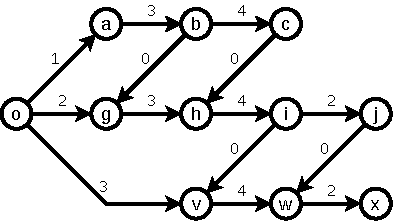
\includegraphics[width=.7\textwidth]{img/event_graph.pdf}
\end{center}
\end{figure}

The time of the event $x$ in the even graph can be calculate as the longest path from origin $o$ to $x$, $\mathrm{T}(x) = \mathrm{L_{max}}(o,\ x)$.


Finding all of the paths from $o$ to each $x \in V$ would be very expensive, by DFS the complexity is exponential \cite{homer2011computability}.

First optimization is the use of Bellman principle \cite{light2024principle}\cite{bellman1952dynamic},

\begin{equation}
	\mathrm{T}(v) = \mathrm{L_{max}}(o,\ v) = \max_{u \in \inver(v)} \mathrm{L_{max}}(o,\ u) + w_{(u,\ v)}.
\end{equation}

This is principle is used by the Floyd-Warshall algorithm \cite{floyd1962algo} and Dijkstra's algorithm \cite{Dijkstra1959} which are used for finding shortest paths for all pairs for vertices and from a select starting vertex respectively. Both of them could be adjusted to find the longest path within polynomial complexity, $\mathrm{O}({|V|}^3)$ for Floyd-Warshall and $\mathrm{O}((|V| + |E|)log|V|)$ for Dijkstra with binary heap.

Since we already use algorithm \ref{alg:toposort} to detect a cycle, we can just process the time of the nodes in the topological order.

\begin{definition}
Critical path $\mathrm{CP}(\cdot)$ for vertex $v$ is the longest path from origin $o$ to $v$.
\end{definition}

Critical path  is limiting the earliest start of event $v$, delaying any event along this path will also delay the event $v$,

\begin{equation}
	\mathrm{L}(\mathrm{CP}(v)) = \mathrm{T}(v).
\end{equation}

\begin{definition}
Critical path edge $\mathrm{CPE}(\cdot)$ of $v$ is the last edge of the critical path for $v$.
\end{definition}

We can again use the Bellman principle to reconstruct the critical path,
\begin{equation}
	\mathrm{CP}(v) = \mathrm{CP}(u) \cup \{(u,\ v)\},\ \mathrm{CPE}(v) = (u,\ v).
\end{equation}

Algorithm \ref{alg:time} outputs the time $\mathrm{T}(\cdot)$ and critical path edge $\mathrm{CPE}(\cdot)$ for each vertex in the event graph. It runs in $\mathrm{O}(|V| + |E|)$ time complexity.

\begin{remark}
In our event graph, the first vertex in the topological order will always be the origin $o$ as it is the only vertex $v$ with $\indeg(v) = 0$.
\end{remark}

\begin{algorithm}[float, caption={Time and critical path predecessor calculation}, label={alg:time}]
input: weighted graph G, topological order O
output: time T and critical path edge CPE for each vertex in G

begin
  foreach v $\in$ V(G)
    T(v) $\gets$ 0
    CPE(v) $\gets$ Undefined
  end

  foreach u $\in$ O $\setminus$ {o}
    foreach (u, v) $\in \outedges$(u)
      if T(v) < T(u) + w$_{u,v}$
        T(v) $\gets$ T(u) + w$_{u,v}$
        CPE(v) $\gets$ (u, v)
      end
    end
  end
end
\end{algorithm}

\paragraph{Example} For event graph in figure \ref{fig:event_graph}, the time and critical path edge output from algorithm \ref{alg:time} is in table \ref{tab:time_crit}. So the vertices in the critical path for $a$ are ($o$, $a$, $b$, $c$), for $j$ are ($o$, $a$, $b$, $c$, $h$, $i$, $j$) and for $w$ are ($o$, $a$, $b$, $c$, $h$, $i$, $u$, $v$, $w$).

\begin{table}[htbp!]
\begin{center}
\caption{Time and critical path edge for vertices in example from figure \ref{fig:event_graph}}\label{tab:time_crit}
\begin{tabular}{lrc}
\toprule
vertex & T & CPE \\
\midrule
a & 1 & (o, a) \\
b & 4 & (a, b) \\
c & 8 & (b, c) \\
g & 4 & (b, g) \\
h & 8 & (c, h) \\
i & 12 & (h, i) \\
j & 14 & (i, j) \\
u & 12 & (i, u) \\
v & 16 & (u, v) \\
w & 18 & (v, w) \\
\bottomrule
\end{tabular}
\end{center}
\end{table}

\chapter{Methodology}

\section{Problem description}
Most of the problem description is taken from the \emph{DISPLIB format specification} \cite{kloster2025displibspec}, a concise explanation is in accompanied paper \cite{kloster2025displiblibrarytraindispatching}.

Each instance in the \emph{DISPLIB} library consist of set of trains and an objective to be minimized. All data is presented in JSON format \cite{pezoa2016foundations}. Train is defined by an operation graph which is DAG, operation has the following content:

\begin{itemize}
    \item minimal duration
    \item start lower bound (optional)
    \item start upper bound (optional)
    \item list of successors
    \item list of required resources
    \begin{itemize}
        \item resource name
        \item release time
    \end{itemize}
\end{itemize}    

Data \ref{data:op} show and example of an operation entry in the instance JSON.

All operation graphs have one entry (start) operation, with no predecessors, and one exit (end) operation, with no successors. Each operation ends exactly when the successor operation starts, exit operation has no end. 

Resources are anything that is required by the operation, typically physical sections of the railway network. Resources can only be used by one operation at the time and are released after the end of the operation that uses it plus the defined release time.

Objective is defined by a list of objectives components, each with the following content 

\begin{itemize}
    \item train
    \item operation
    \item threshold
    \item coefficient (linear objective)
    \item increment (stepwise objective)
\end{itemize}

\begin{remark}
While the format allows both coefficient and increment to be non-zero, in practice none of the instances mix both in one objective component.
\end{remark}

Data \ref{data:obj} show and example of an objective component entry in the instance JSON.

The total objective $J$ is defined as a sum of components for active operations only,

\begin{equation}
J = \sum_{o \in O_{a,J}} c_o \max\{0, t_o - \bar{t}_o\} + d_o H(t_o - \bar{t}_o),
\end{equation}

where $O_{a,J}$ is a set of active operations that have an objective component, $t_o$ is start of the operation, $\bar{t}_o$ is the threshold for the operation, $c_o$ is the linear objective coefficient, $d_o$ is the stepwise objective increment, and $H(\cdot)$ is Heaviside step function \cite{abramowitz1972handbook}.

A solution to the problem is a sequence of events, each event entry corresponds to start of an operation and contains:
\begin{itemize}
    \item train
    \item operation
    \item time
\end{itemize}

Solution is also presented in a JSON format, data \ref{data:events} shows truncated solution example. To reiterate, the end event of an operation is the start event of its successor.

\begin{displaycquote}[Feasible solution requirements in \emph{DISPLIB} format specification]{kloster2025displibspec}
    \begin{itemize}
        \item The sequence of events is given in chronological order, i.e., the time of each event is greater than or equal to the time of all preceding events.
        \item The subsequence of operations applying to each train forms a path through that train’s operations graph, starting at the entry operation and ending at the exit operation.
        \item The time value of each start event satisfies the lower and upper bounds on the start time of the operation.
        \item The duration from each start event to the corresponding end event must be greater than or equal to the minimum duration of the corresponding operation.
    \item For any pair of operations $o_1$ and $o_2$, where:
        \begin{itemize}
            \item the start event of $o_1$ precedes the start event of $o_2$ in the global sequence, and $o_1$ and $o_2$ belong to different trains, and
            \item $o_1$ and $o_2$ use a common resource $r$,
        \end{itemize}
        the following must hold:
        \begin{itemize}
            \item the end event for $o_1$ precedes the start event for $o_2$ in the global sequence, and
            \item the duration from the end event of $o_1$ to the start event of $o_2$ is greater than or equal to the release time of resource $r$ in $o_1$.
        \end{itemize}
    \end{itemize}
\end{displaycquote}

While the events in the solution have a time, their order in the list is still significant, as they define in which order the resources are unlocked and locked. This is to prevent a resource swap situation described in section \ref{sec:swap}.

\subsection{Example problem}
To illustrate the format we have prepared example problem, the railway network diagram is in picture \ref{fig:railway_example}. The network consists of 3 trains, 18 operations, and 8 railway sections, corresponding to resources.

\begin{figure}[htbp!]
\caption{Example railway network}
\label{fig:railway_example}
\begin{center}
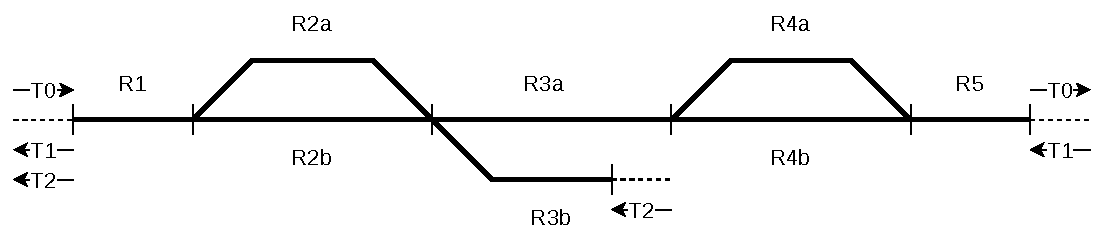
\includegraphics[width=\textwidth]{img/displib_example.pdf}
\end{center}
\end{figure}


The corresponding operation graph for train 0 (first) is in figure \ref{fig:train_dag}, JSON entry for operation 4 is in data \ref{data:op}, and JSON entry for objective component for the last operation is in data \ref{data:obj}.

\begin{figure}[htbp!]
\caption{Operation graph for train 0}
\label{fig:train_dag}
\begin{center}
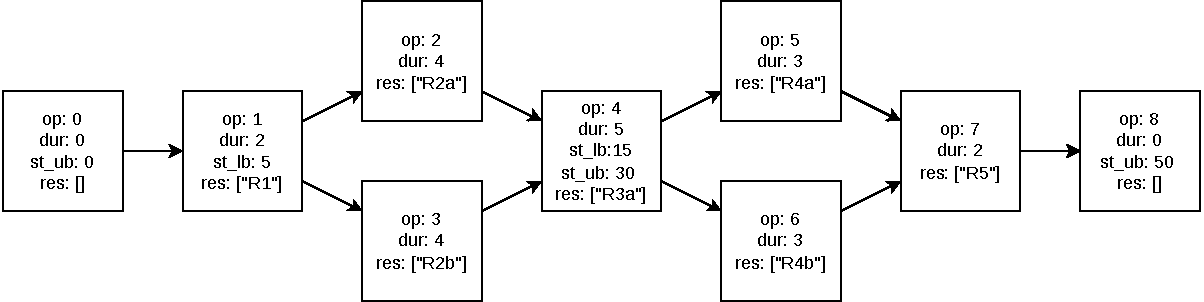
\includegraphics[width=\textwidth]{img/train_dag.pdf}
\end{center}
\end{figure}

\begin{data}[float, caption={JSON operation entry}, label=data:op]
{
    "start_lb": 0,
    "start_ub": 50,
    "min_duration": 5,
    "resources": [
        {
            "resource": "R3a",
            "release_time": 0
        }
    ],
    "successors": [
        5,
        6
    ]
}
\end{data}
\begin{data}[float, caption={JSON objective component entry}, label=data:obj]
{
    "type": "op_delay",
    "train": 0,
    "operation": 8,
    "threshold": 25,
    "coefficient": 1
}
\end{data}

\begin{data}[float, caption={JSON solution truncated}, label=data:events]
{
    "events": [
        ...,
        {
            "train": 0,
            "operation": 5,
            "time": 15
        },
        {
            "train": 1,
            "operation": 4,
            "time": 15
        },
        ...
    ],
    "objective_value": 25
}
\end{data}


\FloatBarrier

\subsection{Resource swap}
\label{sec:swap}

Consider the situation as in figure \ref{fig:swap_railway}, where 2 trains A and B are passing a section of 2 resources X and Y in opposite direction. If we were to set events A2 and B2 to the same time, we would not have a resource collision on either resources (overlap of intervals for operations A1 and B2 on resource X or A2 and B1 on resources Y) but in reality the trains would collide. 

\begin{figure}[htbp!]
\caption{Resource swap railway}
\label{fig:swap_railway}
\begin{center}
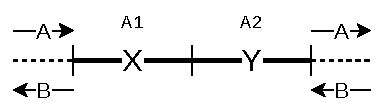
\includegraphics[width=.5\textwidth]{img/swap_railway.pdf}
\end{center}
\end{figure}

In this situation, resource Y is being acquired by A while holding X and X is being required by B while holding Y.

We can detect the resource swaps using an event graph by cycle detection, like in figure \ref{fig:swap_event} where A2 and B2 form a cycle.

\begin{figure}[htbp!]
\caption{Resource swap event graph}
\label{fig:swap_event}
\begin{center}
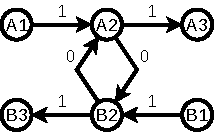
\includegraphics[width=.5\textwidth]{img/swap_event_graph.pdf}
\end{center}
\end{figure}

\begin{remark}
Using cycles in event graph to detect resource swaps only works if all resource precedence edges are present, otherwise we still might have a resource swap situation because the current event times do not create a collision and one or both of the edges that would create the cycle in the event graph are missing.
\end{remark}



% \chapter{Results}

\subsubsection{Instance grouping}
Because the DISPLIB has 112 instances, we split them into 10 groups with approximately the same size (9 to 16 instance per group) based in their initial source (encoded in the name), which also corresponds to the structure of the problem. Unless specified otherwise, the presented results will be the median across the instances inside the group, we feel that this number should be a good representation of the results as it will not be skewed by a single instance within the group and thus provide us with a valid overview that can still be distinguished between the groups.	

\section{Preprocessing}
To gauge how well did the aggregation of the instance 


\begin{table}[htbp!]
\begin{center}
\caption{Initial instance data}
\input{tables/instance_data.tex}
\label{tab:instance_data}
\end{center}
\footnotesize $^\mathrm{a}$Operation to resource relations, will be compared to resource chunks.
\end{table}

% \include{15conlusion}
% \chapter{Dummy}

\begin{figure}[htbp!]
\caption{Náhodný výběr z~rozdělení $\mathcal{N}_2(\boldsymbol{0},\,I)$}
\label{obr03:Nvyber}
\begin{center}
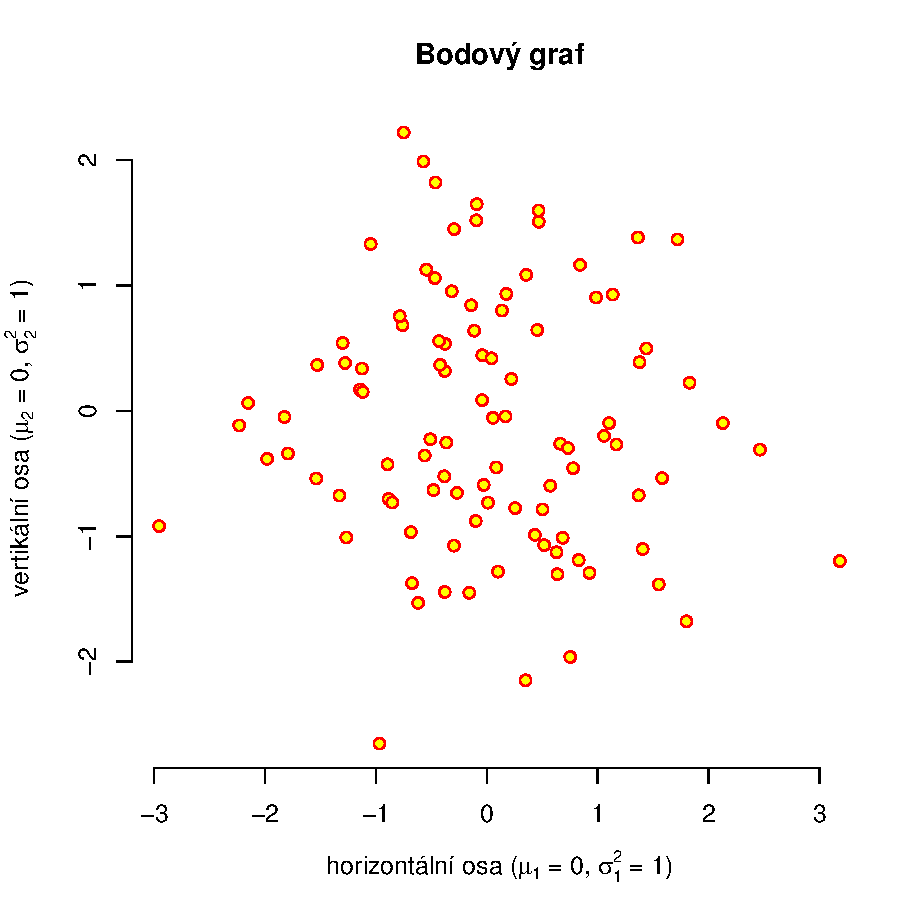
\includegraphics[width=.525\textwidth]{img/ukazka-obr01}
% Příponu není potřeba explicitně uvádět, pdflatex automaticky hledá pdf.
% Rozměry také není nutné uvádět.
\end{center}

\footnotesize \textit{Poznámka:} 
Vlastní zpracování na základě dat z ČSÚ.
\end{figure}

\begin{table}[htbp!]

\begin{center}
%%% Tabulka používá následující balíčky:
%%%   - booktabs (\toprule, \midrule, \bottomrule)
%%%   - dcolumn (typ sloupce D: vycentrovaná čísla zarovnaná na
%%%     desetinnou čárku
%%%     Všimněte si, že ve zdrojovém kódu jsou desetinné tečky, ale
%%%     tisknou se čárky.

\caption{Maximálně věrohodné odhady modelů 1 a 2}\label{tab03:Nejaka}
\begin{tabular}{lrr}
\toprule
              & \multicolumn{1}{c}{\textbf{1}} & \multicolumn{1}{c}{\textbf{2}}\\
\midrule
\multirow{2}{*}{Abs. člen}     &$-10,01$***  &42,01**\\
                               & (1,01)      &(1,89)\\
\multirow{2}{*}{Pohlaví (muž)} &	9,89*       & 8,16\\
                               & (5,98)	    &(8,18)\\
Výška (cm)                	   & 0,78***     &(0,12)	\\
\bottomrule
\end{tabular}
\end{center}

\footnotesize \textit{Poznámka:} 
(i) V závorkách jsou uvedeny směrodatné chyby získané na základě 500 iterací neparametrického bootstrapu.\\
(ii) * p < 0,05, ** p < 0,01, *** p < 0,001.\\
(iii) Vlastní zpracování na základě dat z ČSÚ.
\end{table}

\begin{code}{Python}{Ukázka zpracování pomocí Pythonu}{zpracovani-python}
import numpy as np
    
def incmatrix(genl1,genl2):
    m = len(genl1)
    n = len(genl2)
    M = None #to become the incidence matrix
    VT = np.zeros((n*m,1), int)  #dummy variable
    
    #compute the bitwise xor matrix
    M1 = bitxormatrix(genl1)
    M2 = np.triu(bitxormatrix(genl2),1) 

    for i in range(m-1):
        for j in range(i+1, m):
            [r,c] = np.where(M2 == M1[i,j])
            for k in range(len(r)):
                VT[(i)*n + r[k]] = 1;
                VT[(i)*n + c[k]] = 1;
                VT[(j)*n + r[k]] = 1;
                VT[(j)*n + c[k]] = 1;
                
                if M is None:
                    M = np.copy(VT)
                else:
                    M = np.concatenate((M, VT), 1)
                
                VT = np.zeros((n*m,1), int)
    
    return M
\end{code}

% \include{tabulky-obrazky}
% \include{prace-s-prameny}
% \include{pdf-a}
% \include{...}
% \include{...}
{%
\pagestyle{plain}
%% Toto platí v případě použití samostatné bibliografické databáze
\printbibliography[title={\bibnamex},heading={bibintoc}]

}


%%% Přílohy k práci, existují-li. Každá příloha musí být alespoň jednou
%%% odkazována z vlastního textu práce. Přílohy se číslují.
%%% Attachments to thesis, if any. Each attachment must be referenced at 
%%% least once in your own text. The appendices are numbered.
% \part*{\Prilohy\thispagestyle{empty}}
% \appendix
% \include{21app}
% \include{22app}
% \include{...}
% \include{...}

\end{document}
